\documentclass{article}

% Language setting
% Replace `english' with e.g. `spanish' to change the document language
\usepackage[english]{babel}
\usepackage{subfig}


% Set page size and margins
% Replace `letterpaper' with `a4paper' for UK/EU standard size
\usepackage[letterpaper,top=2cm,bottom=2cm,left=3cm,right=3cm,marginparwidth=1.75cm]{geometry}

% Useful packages
\usepackage{amsmath}
\usepackage{graphicx}
\usepackage[colorlinks=true, allcolors=blue]{hyperref}
\usepackage[utf8]{inputenc}
\usepackage{fancyhdr}

\pagestyle{fancy}
\fancyhf{}
\rhead{Halbach Permanent Magnets}
\lhead{01006 Advanced Engineering Mathematics 1}
\cfoot{\textbf{Page \thepage}}


\begin{document}
\begin{titlepage}
\begin{figure}
\centering

\includegraphics[width=0.3\textwidth]{DTU.logo.png}
\end{figure}
\title{01006 Advanced Engineering Mathematics 1
\vspace{5}
\hline
\\ \vspace{5}
\\ \textbf{Analytical modeling of 2D Halbach Permanent
Magnets - Group 2 }
\\ \vspace{5}
\\ \hline
\vspace{30} } 


\author{\Large Andrea Fratini, s215177
\\\Large Emma Krühne, s215130
\\\Large Jacopo Ceccuti, s215158
\\\Large Isabella del Furia, s215138
\\\Large Madeleine Taylor, s215234
\\\Large Nina Dietz, s215200 \vspace{150}  }
\date{29/04/2022} 
\maketitle
\thispagestyle{empty}
\end{titlepage}
\setcounter{page}{1}

\pagebreak

\section{Introduction}
 Halbach magnets are a type of permanent magnet, which means that their atomic structure consists of having their atoms alligned at all times. They are also a type of electromagnet that generate a homogeneous and relatively large magnetic field from a very small current. In addition, Halbach magnets are linear and consist of N layers stacked outside an outermost core that serve as a fixed magnetic field that follows the cylindrical coordinates - allowing for computations that can be applied to technical analysis. In this assignment, we will utilize these application of these calculations to analyze the mathematical concepts behind the functionality of Halbach magnets.

\section{Cylindrical Coordinates}
To better understand how Halbach magnets work, we will analyze their linear model. What makes it linear, as mentioned in the introduction, is where the magnetic field follows the cylindrical coordinates which provides a natural extension of polar coordinates to three dimensions. In the following section, we explain how cylindrical coordinates can be used for the analysis of Halbach magnets. 

\subsection{Exercise 1}
In this exercise we are asked to show that the base vectors can be written as a function of rectangular coordinates in the following way:
\begin{equation}
    \mathbf{e}_r = (x^2+y^2)^-1/2 (x,y,0)
\end{equation}
\begin{equation}
    \mathbf{e}_\theta = (x^2+y^2)^-1/2 (-y,x,0)
\end{equation}
\begin{equation}
    \mathbf{e}_z = (0,0,1)
\end{equation}

In doing so, we use the following polar coordinates:
\[x = r cos(\theta)\]
\[y = r sin(\theta)\]
\[z = z\]
Initially, we know that the base vectors can be rewritten as:
\begin{equation}
\mathbf{e}_r = k_a(x,y,0)
\end{equation}
\begin{equation}
\mathbf{e}_\theta = k_b(-y,x,0)
\end{equation}
\begin{equation}
\mathbf{e}_z = (0,0,1)
\end{equation}
We also recognize that:
\begin{equation}
\mathbf{e}_{base} = (\mathbf{e}_r, \mathbf{e}_\theta,\mathbf{e}_z)
\end{equation}
This is an orthonormal basis. And for these vectors to make up an orthonormal basis, all of their lengths must be equal to 1. Now from here, we can find the equation representing the length of each of the above three vectors and set it equal to 1, to then solve for the constants ka and kb.
In doing so we get:
\begin{equation} \label{eq:8}
    {| \mathbf{e}_{r}|}=k_{a}{| \mathit{(x\,,y\,,0)\,}|}\Rightarrow k_{a}\sqrt{x^{2}+y^{2}}=1\Rightarrow k_{a}=\frac{\textcolor{MediumSeaGreen}{1}}{\sqrt{x^{2}+y^{2}}}
\end{equation}
\begin{equation} \label{eq:9}
    {| \mathbf{e}_{\theta}|}=k_{b}{| \mathit{(-y\,,x\,,0)\,}|}\Rightarrow k_{b}\sqrt{(-y)^{2}+x^{2}}=1\Rightarrow k_{b}=\frac{\textcolor{MediumSeaGreen}{1}}{\sqrt{x^{2}+y^{2}}}
\end{equation}
\begin{equation}
    {| \mathbf{e}_{z}|}=1
\end{equation}
Now we can plug the values for ka and kb into the base vector equations written above to get:
\begin{equation*}
    \mathbf{e}_{r}=\frac{1}{\sqrt{x^{2}+y^{2}}}(x ,y ,0)
\end{equation*}
\begin{equation}
    \mathbf{e}_{\theta}=\frac{1}{\sqrt{x^{2}+y^{2}}}(-y ,x ,0)
\end{equation}
\begin{equation} \label{eq:12}
    \mathbf{e}_{z}=(0,0,1)
\end{equation}
And thus we have proven that the new basis vectors may be written as a function of rectangular coordinates in the given way.

\subsection{Exercise 2}
This exercise asks to show that the basis vectors
\begin{equation}
(\mathbf{e}_r, \mathbf{e}_\theta, \mathbf{e}_z)
\end{equation}
expressed by cylindrical coordinates, are given by:
\begin{equation}
\mathbf{e}_r = (cos(\theta), sin(\theta), 0)
\end{equation}
\begin{equation}
\mathbf{e}_\theta = (-sin(\theta), cos(\theta), 0)
\end{equation}
\begin{equation}
\mathbf{e}_z = (0,0,1)
\end{equation}
To do so, we substitute the values for x, y, and z given in exercise 1 into equations \ref{eq:8} and \ref{eq:9} from exercise 2 that represent the 3 basis vectors.
\begin{equation}
    e_{r}= \frac{1}{\sqrt{(r cos(\theta))^2+(r sin(\theta))^2}}(r cos(\theta), r sin(\theta),0)
\end{equation}
\begin{equation}
    e_{\theta}= \frac{1}{\sqrt{(r cos(\theta))^2+(r sin(\theta))^2}}(-r sin(\theta), r cos(\theta),0) 
\end{equation}
After doing so, we realize that these equations can be simplified using the Pythagorean trigonometric identity which states: \[\cos(\theta)^{2}+\sin(\theta)^{2}=1\]. And thus we have the following:
\begin{equation}
    e_{\theta}= \frac{1}{\sqrt{(r^2)}}(r cos(\theta), r sin(\theta),0) \Rightarrow e_{r} = (cos(\theta),sin(\theta),0)
\end{equation}
\begin{equation}
    e_{\theta}= \frac{1}{\sqrt{(r^2)}}(-r sin(\theta), r cos(\theta),0) \Rightarrow e_{\theta} = (-sin(\theta),cos(\theta),0)
\end{equation}
\begin{equation}
    \mathbf{e}_z = (0,0,1)
\end{equation}
For this last equation representing $\mathbf{e}_z$ we don't substitute values like we did for the other two basis vectors. Instead, we can recognize that the length of the vector is 1, and so when we normalize it, we are just dividing the values that make up the vector by 1. And since dividing any value by 1 doesn't change the value, $\mathbf{e}_z$ maintains the same value as written in line 12.







\subsection{Exercise 3}
Here we are asked to find an expression for the partial derivative of the function \emph{f} with respect to \emph{r} and show that:
\[\frac{\partial f}{\partial r} = \nabla f \cdot \mathbf{e}_r\]
To do so, we take both sides of the equation into consideration and demonstrate that they are equal to one another.
Firstly, we know from line 12 in the given exercises that the gradient of a function \emph{f} is defined as:

\begin{equation}
\nabla f(x,y,z) =( \frac{\partial f}{\partial x}, \frac{\partial f}{\partial y}, \frac{\partial f}{\partial x})
\end{equation}
By then calculating the dot product of $\nabla f(x,y,z)$ and $\mathbf{e}_r$ we get:
\begin{equation} \label{eq:23}
\left[\begin{array}{c}
\frac{\partial f}{\partial x} 
\\
 \frac{\partial f}{\partial y} 
\\
 \frac{\partial f}{\partial z} 
\end{array}\right]
\cdot
\left[\begin{array}{c}
\cos (\theta) 
\\
 \sin (\theta) 
\\
 0 
\end{array}\right]
= \frac{\partial f}{\partial x}(\cos (\theta))+\frac{\partial f}{\partial y}(\sin (\theta)) + 0
\end{equation}
Now we compare this right hand side of the equation to the left hand side of the equation. But first we must analyze the left hand side of the equation which can be expressed as: 
\begin{equation}
\frac{\partial f}{\partial r} = \frac{\partial }{\partial r} ((f(x,y,z))
\end{equation}
And from the gradient, we see that the partial derivatives of the x,y,z components of $f(x,y,z)$ with respect to $r$ are:
\begin{equation}
\frac{\partial x}{\partial r} = \cos \theta
\end{equation}
\begin{equation}
\frac{\partial y}{\partial r} = \sin \theta
\end{equation}
\begin{equation}
\frac{\partial z}{\partial r} = 0
\end{equation}
\\
Since equation \ref{eq:23} is a composite function, the chain rule, as it is defined in the theorem 19.46, eNote 19, can subsequently be applied:
\begin{equation}
\frac{\partial f}{\partial r} = \frac{\partial f}{\partial x}\frac{\partial x}{\partial r}+\frac{\partial f}{\partial y}\frac{\partial y}{\partial r}+\frac{\partial f}{\partial z}\frac{\partial z}{\partial r}
\end{equation}
We can then substitute what we found for the partial derivatives of the x,y,z components of $f(x,y,z)$ with respect to $r$ in the above expressions to get: 
\begin{equation}
    \frac{\partial f}{\partial r} = \frac{\partial f}{\partial x}(cos(\theta))+\frac{\partial f}{\partial y}(\sin(\theta))
\end{equation}
And because both sides of the equation are equal, we find and thus prove that:
\begin{equation}
    \frac{\partial f}{\partial r} = \nabla f \cdot \mathbf{e}_r
\end{equation}

\subsection{Exercise 4}
In this exercise we are asked to use the same method as we did for exercise 3, but instead show that:
\[\frac{\partial f}{\partial \theta} = r\nabla f \cdot \mathbf{e}_\theta\]
We first consider the left hand side of the equation, $\frac{\partial f}{\partial \theta}$. As demonstrated in the previous exercise, because $\frac{\partial f}{\partial \theta} =\frac{\partial }{\partial \theta} (f(x,y,z))$ is a composite function the chain rule can be applied, so that we now we have the equation:
\begin{equation} \label{eq:31}
\frac{\partial f}{\partial \theta} = \frac{\partial f}{\partial x}\frac{\partial x}{\partial \theta}+\frac{\partial f}{\partial y}\frac{\partial y}{\partial \theta}+\frac{\partial f}{\partial z}\frac{\partial z}{\partial \theta}
\end{equation} 
Then finding the partial derivatives of the x,y,z components of $f(x,y,z)$ with respect to $\theta$:
\begin{equation}
\frac{\partial x}{\partial \theta} = -rsin \theta
\end{equation}
\begin{equation}
\frac{\partial y}{\partial \theta} = r\cos\theta
\end{equation}
\begin{equation}
\frac{\partial z}{\partial \theta} = 0
\end{equation}
 Substituting these values into \ref{eq:31}, we find:
\begin{equation}
\frac{\partial f}{\partial \theta} = \frac{\partial f}{\partial x}(-rsin \theta) + \frac{\partial f}{\partial y}(r\cos\theta)
\end{equation} 
Now we can consider the right side of the equation, $ r\nabla f \cdot \mathbf{e}_\theta\ $which can be written as the following:
\begin{equation}
    r\nabla f \cdot \mathbf{e}_\theta\ = 
    \left[\begin{array}{c}
    \frac{\partial f}{\partial x} 
    \\
     \frac{\partial f}{\partial y} 
    \\
     \frac{\partial f}{\partial z} 
    \end{array}\right]
    \cdot
    \left[\begin{array}{c}
    -\sin (\theta) 
    \\
     \cos (\theta) 
    \\
     0 
    \end{array}\right]
\end{equation} 
Which can be simplified as:
\begin{equation}
    r\nabla f \cdot \mathbf{e}_\theta\ = r\cdot\frac{\partial f}{\partial x}(-sin (\theta))+r\cdot\frac{\partial f}{\partial y}(\cos (\theta)) + 0
\end{equation}
Thus, as that both sides of the equation are equal to each other, we have proven that $\frac{\partial f}{\partial \theta} = r\nabla f \cdot \mathbf{e}_\theta$. 

\subsection{Exercise 5}
In this exercise we are asked to show using our results from exercises 3 and 4 that:
\begin{equation}
    \nabla f\left(r,\theta,z\right)=\frac{\partial f}{\partial r}\mathbf{e}_{r}+\frac{1}{r}\frac{\partial f}{\partial \theta}\mathbf{e}_{\theta}+\frac{\partial f}{\partial z}\mathbf{e}_{z}
\end{equation}
The general equation for the gradient of a function, as given in exercise 2, is:
\begin{equation}
    \nabla f\left(x,y,z\right)=\left(\frac{\partial f}{\partial x},\frac{\partial f}{\partial y},\frac{\partial f}{\partial z}\right)
\end{equation}
Now reapplying this equation to our cylindrical coordinate variables:
\begin{equation}
    \nabla f\left(r,\theta,z\right)=\left(\frac{\partial f}{\partial r},\frac{\partial f}{\partial\theta},\frac{\partial f}{\partial z}\right)
\end{equation}
Using our work from exercise 3, we know that $\frac{\partial f}{\partial r}=\nabla f\cdot \mathbf{e}_{r}$ In addition, from our work in exercise 4 we also know that $\frac{\partial f}{\partial \theta}=r\cdot \nabla f\cdot \mathbf{e}_{\theta}$.
From the equation $\frac{\partial f}{\partial z}= \nabla f\cdot \mathbf{e}_{z}$, we can utilize the same approach as used in exercises 3 and 4 to find $\frac{\partial f}{\partial z}$ by finding the partial derivatives of the x,y,z components of $f(x,y,z)$ in respect to z:
\begin{equation}
    \frac{\partial x}{\partial z}=0
\end{equation}
\begin{equation}
    \frac{\partial y}{\partial z}=0
\end{equation}
\begin{equation}
    \frac{\partial z}{\partial z}=1
\end{equation}
These three expressions make up the coordinates of $\mathbf{e}_z$ as shown in equation \ref{eq:12} exercise 2: (0, 0, 1). From here:
\begin{equation}
    \nabla f \cdot \mathbf{e}_z\ = 
    \left[\begin{array}{c}
    \frac{\partial f}{\partial x} 
    \\
     \frac{\partial f}{\partial y} 
    \\
     \frac{\partial f}{\partial z} 
    \end{array}\right]
    \cdot
    \left[\begin{array}{c}
    0
    \\
     0
    \\
     1
    \end{array}\right]
    = \frac{\partial f}{\partial z}
\end{equation}
We therefore find that both sides of the equation are equal and thus, $\frac{\partial f}{\partial z} =  \nabla f \cdot \mathbf{e}_z$.
\\
From here, we use equation 13 given in the exercises from exercise 2, $\nabla f=\nabla f_{r} \mathbf{e}_{r}+\nabla f_{\theta}\mathbf{e}_{\theta}+\nabla f_{z} \mathbf{e}_{z}$, and can substitute $\frac{\partial f}{\partial r}$ for $\nabla f_r$ as that $ \nabla f_r =\nabla f\cdot \mathbf{e}_{r}$ (from equation 14 in exercise 2 in the given text). Therefore, $\nabla f_{r}=\frac{\partial f}{\partial r}$.
\\
We can next substitute $\frac{\partial f}{\partial z}$ for $\nabla f_z$ as that $ \nabla f_z =\nabla f\cdot \mathbf{e}_{z}$, according to equation 14 of the given exercises in exercise 2.
\\
Finally we can substitute $\frac{1}{r}\frac{\partial f}{\partial \theta}$ for $\nabla f_{\theta}$ as that $\nabla f_{\theta}=\nabla f\cdot \mathbf{e}_{\theta}$, also based on equation 14 of the given exercises in exercise 2. Because $\frac{\partial f}{\partial \theta}$ = $r\nabla f\cdot \mathbf{e}_{\theta}$, we must multiply $\frac{\partial f}{\partial \theta}$ by $\frac{1}{r}$ to have it equate to $\nabla f_{\theta}$. 
\\ 
After completing all the above substitutions into the given equation 13 we find:
\begin{equation}
    \nabla f\left(r,\theta,z\right)=\frac{\partial f}{\partial r}\mathbf{e}_{r}+\frac{1}{r}\frac{\partial f}{\partial\theta}\mathbf{e}_{\theta}+\frac{\partial f}{\partial z}\mathbf{e}_{z}
\end{equation}

\subsection{Exercise 6}
In this exercise we let $f(x,y,z)$ be a function and let $\mathbf{V}(x,y,z)$ be a vector field. We are asked to show that following equation is true:
\begin{equation}
    \mathbf{Div}(f\mathbf{V})= \nabla f\cdot \mathbf{V}+\mathit{f \mathbf{Div}}\left(\mathbf{V}\right)
\end{equation}
We can begin by first considering the left hand side of the equation. We know from eNote 19, definition 19.44, the gradient of $f$ is defined as:
\begin{equation}
    \nabla f=(\frac{\partial }{\partial x}\mathbf{e}_{x},\frac{\partial}{\partial y}\mathbf{e}_{y},\frac{\partial}{\partial z}\mathbf{e}_{z})
\end{equation}
We also know from eNote 26, definition 26.18, that the divergence of a vector field $\mathbf{V}$ is defined as:
\begin{equation}
    \mathbf{Div}\left(\mathbf{V}\right)=\nabla \cdot \mathbf{V}=\frac{\partial}{\partial x}{V}_{x}+\frac{\partial}{\partial y}{V}_{y}+\frac{\partial}{\partial z}{V}_{z}
\end{equation}
Now expanding the left hand side, while following the general definition of divergence, it can be rewritten as:
\begin{equation}
    \mathbf{Div}\left(\mathit{f\mathbf{V}}\right)=\frac{\partial}{\partial x}\left(\mathit{f\mathbf{V}}_{x}\right)+\frac{\partial}{\partial y}\left(\mathit{f\mathbf{V}}_{y}\right)+\frac{\partial}{\partial z} \left(\mathit{f\mathbf{V}}_{z}\right)
\end{equation}
We can now apply the product rule, as mentioned above, as this is the sum of the derivatives of 3 composite functions:
\begin{equation} \label{eq:50}
    \mathbf{Div}\left(\mathit{f\mathbf{V}}\right)=\frac{\partial V_x}{\partial x}f+\frac{\partial f}{\partial x}V_{x}+\frac{\partial V_y}{\partial y}f+\frac{\partial f}{\partial y}V_{y}+\frac{\partial V_z}{\partial z}f+\frac{\partial f}{\partial z}V_{z}
\end{equation}
From our definition of the gradient of $f$, it can be understood that the terms of our equation \ref{eq:50} that are multiplied with the x,y,z components of the vector field $\mathbf{V}$ correspond with $\nabla f \cdot \mathbf{V}$. It can also be understood that the partial derivatives of the x,y,z components of the vector field $\mathbf{V}$ multiplied by $f$ correspond to the $\mathbf{Div}(\mathbf{V})f$.
\\
\\
Thus the left hand and right hand sides of the equation are equal to each other, and the equation $ \mathbf{Div}(f\mathbf{V})= \nabla f\cdot \mathbf{V}+\mathit{f \mathbf{Div}}\left(\mathbf{V}\right)$ is true. 

\subsection{Exercise 7}
In this exercise we were told to find the divergence of the 3 basis vectors $(\mathbf{e}_r, \mathbf{e}_\theta,\mathbf{e}_z)$, and determine why two of these are zero. 
\\
To find the divergence of these basis vectors where:
\[\mathbf{e}_r = (cos(\theta), sin(\theta), 0)\]
\[\mathbf{e}_\theta = (-sin(\theta), cos(\theta), 0)\]
\[\mathbf{e}_z = (0,0,1)\]
Utilizing definition 26.18 from the eNotes, we can find the divergence of the basis vector $\mathbf{e}_r$ to be (see appendix 1, subsection 1):
\begin{equation}
  \frac{2}{\sqrt{x^{2}+y^{2}}}-\frac{x^{2}}{\left(x^{2}+y^{2}\right)^{\frac{3}{2}}}-\frac{y^{2}}{\left(x^{2}+y^{2}\right)^{\frac{3}{2}}}
\end{equation}
This then simplifies to be:
\begin{equation}
   \frac{1}{\sqrt{x^{2}+y^{2}}}
\end{equation}
As this is a non-zero divergence, we are told to put this into cylindrical coordinates (see appendix 1, subsection 4), where $x = rcos(\theta)$ and $y = rsin(\theta)$:
\begin{equation}
    \frac{1}{\sqrt{r^{2} \cos \left(\theta\right)^{2}+r^{2} \sin \left(\theta\right)^{2}}}
\end{equation}
Which when factorized:
\begin{equation}
    \frac{1}{\sqrt{r^{2} \left(\cos \left(\theta\right)^{2}+\sin \left(\theta\right)^{2}\right)}}
\end{equation}
The non-zero divergence in cylindrical coordinates thus simplifies to $\frac{1}{r}$ due to the Pythagorean trigonometric identity where $\cos^{2}\left(\theta\right)+\sin^{2}\left(\theta\right)=1$.
\\
We then take the divergence of $\mathbf{e}_\theta$ (see appendix 1, subsection 2), which we find to be:
\begin{equation}
    \frac{y x}{\left(x^{2}+y^{2}\right)^{\frac{3}{2}}}  -\frac{y x}{\left(x^{2}+y^{2}\right)^{\frac{3}{2}}} + 0
\end{equation}
This simplifies to be zero due to the opposite signs in the equation.
\\
The divergence of $\mathbf{e}_z$ is also zero (see appendix 1, subsection 3) as that the differentiation of an expression with no variables is always zero. 
\\
What we can observe from this is that the vector field of $\mathbf{e}_r$ is an explosion field, as that it has a positive divergence, and that the vector fields of both $\mathbf{e}_\theta$ and $\mathbf{e}_z$ are constant vector fields as that they have divergences of zero. 



\subsection{Exercise 8}
We know from line 18 in the given exercises that $\mathbf{V}$ can be defined as the expression:
\begin{equation}
    \mathbf{V} = V_{r}\mathbf{e}_{r}+V_{\theta}\mathbf{e}_{\theta}+V_{z}\mathbf{e}_{z}
\end{equation}
From the definition of divergence given in eNote 26, definition 26.18, we wan write $\mathbf{Div}\mathbf{(V)}$ as the following:
\begin{equation}
    \mathbf{Div}\mathbf{(V)} = \nabla (V_r\mathbf{e}_r)+\nabla (V_\theta\mathbf{e}_\theta)+\nabla (V_z\mathbf{e}_z)
\end{equation}
First considering $\nabla (V_r\mathbf{e}_r)$, as that it is a composite function it can be written out as:
\begin{equation}
    \nabla (V_r\mathbf{e}_r) = V_r(\nabla \mathbf{e}_r) + (\nabla V_r)\mathbf{e}_r
\end{equation}
Considering that $V_r$, the $r$ component of the vector field $\mathbf{V}$, is alike to $f_r$, the $r$ component of the function $f$, we can apply our understanding from exercise 5 to find:
\begin{equation}
    \nabla (V_r\mathbf{e}_r) = V_r \frac{1}{r} +\frac{\partial V_r}{\partial r}
\end{equation}
Using the same method as above, $\nabla (V_\theta\mathbf{e}_\theta)$ can be found to be:
\begin{equation}
     \nabla (V_\theta \mathbf{e}_\theta) = V_\theta(\nabla \mathbf{e}_\theta) + (\nabla V_\theta)\mathbf{e}_\theta
\end{equation}
\begin{equation}
     \nabla (V_\theta\mathbf{e}_\theta) = V_\theta \frac{1}{r} +\frac{\partial V_\theta}{\partial \theta}+0
\end{equation}
Finally, $\nabla (V_z\mathbf{e}_z)$ can be found to be:
\begin{equation}
     \nabla (V_z \mathbf{e}_z) = V_z(\nabla \mathbf{e}_z) + (\nabla V_z)\mathbf{e}_z
\end{equation}
\begin{equation}
     \nabla (V_z\mathbf{e}_z) = \frac{\partial V_z}{\partial z}+0
\end{equation}
Thus, from combining the found expression above, $\mathbf{Div}(\mathbf{V})$ can be expressed as:
\begin{equation}
  \mathbf{Div}\mathbf{(V)}=\frac{V_{r}}{r}+\frac{\partial V_{r}}{\partial  r}+\frac{\partial V_{\theta}}{\partial \theta}\frac{1}{r}+\frac{\partial V_{z}}{\partial z}
\end{equation}
\newpage
\section{Magnetic Field Around a Conductor}
In this section, by using cylindrical coordinates, we will perform calculations to understand and observe magnetic fields inside and outside of a magnet. 
\subsection{Exercise 9}
It is given that the unit for $\mathbf{J}$ is $\frac{A}{m^2}$, where $A$ stands for amperes which  measure of the amount of electric charge in motion per unit time (electrical current, represented by the symbol $I$). $m^2$ represents the cross-sectional area the electric current is flowing through. Because this is a measurement of a wire, the cross sectional area will be that of a circle, where area = $\pi  R^2$. Because the current flows along the unit vector $\mathbf{e}_z$ this means $\mathbf{J}$ must be multiplied by this basis vector.
\\
From this analysis, we get the equation for $\mathbf{J}$ to be:
\begin{equation}
    \emph{\textbf{J}}=\frac{I}{\pi\ R^{2}}\cdot \mathbf{e}_{z}
\end{equation}
Where in the above equation: $I$ is the current, R is the radius, and $\mathbf{e}_{z}$ is the unit vector. It is important to note that if the radial position (represented by little r) is greater than the radius of the conductor(represented by large R) as it can be seen in the figure bellow, then $\mathbf{J}$ is 0 because no current can flow outside a conductive region. 
\begin{figure}[h!]
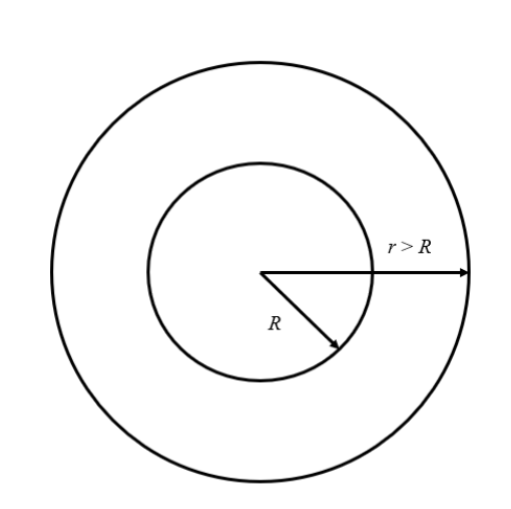
\includegraphics[width=8cm]{radius.PNG}
\centering
\caption{Radius inside and outside the conductor}
\end{figure}
\newpage
\subsection{Exercise 10}
Here we are asked to prove that:$\frac{\partial B_{z}}{\partial \theta}=0$ and $\frac{\partial B_{z}}{\partial r}=0$. We can accomplish this by using equation 21 from the given exercises but replacing $\mathbf{Rot(V)}$ with $\mathbf{Rot(B)}$. In finding this equation we get:
\begin{equation}
    \mathbf{Rot(B)}=\nabla \times \mathbf{B}=\left(\frac{1}{r}\frac{\partial B_{z}}{\partial \theta}-\frac{\partial B_{\theta}}{\partial z}\right)\mathbf{e}_{r}+\left(\frac{\partial B_{r}}{\partial z}-\frac{\partial B_{z}}{\partial r}\right)\mathbf{e}_{\theta}+\left(\frac{\partial B_{\theta}}{\partial r}+\frac{B_{\theta}}{r}-\frac{1}{r}\frac{\partial B_{r}}{\partial \theta}\right)\mathbf{e}_{z}
\end{equation}
In line 23 from the given exercises it is stated that:
\begin{equation}
    \frac{\partial B_{r}}{\partial z}=0,\frac{\partial B_{\theta}}{\partial z}=0,\frac{\partial B_{z}}{\partial z}=0
\end{equation}
Thus, we can simplify to get:
\begin{equation}
    \mathbf{Rot(B)}=\left(\frac{1}{r}\frac{\partial B_{z}}{\partial \theta}-0\right)\mathbf{e}_{r}+\left(0-\frac{\partial B_{z}}{\partial r}\right)\mathbf{e}_{\theta}+\left(\frac{\partial B_{\theta}}{\partial r}+\frac{B_{\theta}}{r}-\frac{1}{r}\frac{\partial B_{r}}{\partial \theta}\right)\mathbf{e}_{z}
\end{equation}
\begin{equation}
      =\left(\frac{1}{r}\frac{\partial B_{z}}{\partial \theta}\right)\mathbf{e}_{r}+\left(\frac{\partial B_{z}}{\partial r}\right)\mathbf{e}_{\theta}+\left(\frac{\partial B_{\theta}}{\partial r}+\frac{B_{\theta}}{r}-\frac{1}{r}\frac{\partial B_{r}}{\partial \theta}\right)\mathbf{e}_{z}
\end{equation}
Then, from exercise 9 we know that $\mathbf{Rot(B)}$ only has components in the z-direction, meaning that the components of $B$ with respect to r and $\theta$ should be zero.
We can then say that:
\begin{equation} \label{eq:70}
    \left(\frac{1}{r}\frac{\partial B_{z}}{\partial \theta}\right)\mathbf{e}_{r}=0 \textrm{ and thus, } \frac{\partial B_{z}}{\partial \theta}=0
\end{equation}
\begin{equation} \label{eq:71}
    \left(\frac{\partial B_{z}}{\partial r}\right)\mathbf{e}_{\theta}=0 \textrm{ and thus, } \frac{\partial B_{z}}{\partial r}=0
\end{equation}
\subsection{Exercise 11}
In this exercise it is asked to write down and solve a differential equation for $B_r(r)$ given that the divergence of $\mathbf{B}$ is equal to 0.
\\
To do this, the divergence of $\mathbf{B}$ first needs to be defined. We can model the divergence of $\mathbf{B}$ after the the divergence of $\mathbf{V}$ given in line 20 in the exercises:
\begin{equation} \label{eq:72}
   \mathbf{Div}(\mathbf{B})=\frac{\partial B_{r}}{\partial r}+\frac{B_{r}}{r}+\frac{1}{r}\frac{\partial B_{\theta}}{\partial \theta}+\frac{\partial B_{z}}{\partial z}=0
\end{equation}
We know from line 23 in the given exercises that $\frac{\partial B_{z}}{\partial z}=0$. We can then 
rewrite the above equation in line \ref{eq:72} as:
\begin{equation}
    \mathbf{Div}(\mathbf{B})=\frac{\partial B_{r}}{\partial r}+\frac{B_{r}}{r}+\frac{1}{r}\frac{\partial B_{\theta}}{\partial\theta}=0 \textrm{ or } \frac{\partial B_{r}}{\partial r}+\frac{B_{r}}{r}=-\frac{1}{r}\frac{\partial B_{\theta}}{\partial \theta}
\end{equation}
From the definition 16.1 in eNote 16, the general formula of differential equation is:
\begin{equation}
    x'\left(t\right)+p\left(t\right)x\left(t\right)=q\left(t\right)
\end{equation}
In the context of the equation for the divergence of $B$:
\begin{equation}
    x'\left(t\right)=\frac{\partial B_{r}}{\partial r},p\left(t\right)=\frac{1}{r},q\left(t\right)=-\frac{1}{r}\frac{\partial B_{\theta}}{\partial \theta}
\end{equation}
As is stated in exercise 10, there is circular symmetry within the magnetic field. Therefore it must not vary as it rotates around the axis of the wire. This means that $\mathbf{B}$ does not depend on  $\theta$. This implies that $\frac{\partial B_ \theta}{\partial \theta} = 0$.
\\
\\
Following theorem 16.9 from eNote 16 to solve for a particular solution, the differential equation should be become homogeneous such that $x \left(t\right)+p\left(t\right)x\left(t\right)=0$. 
\\
Solving the homogeneous equation:
\begin{equation}
    \frac{\partial B_{r}}{\partial r}+\frac{B_{r}}{r}=0
\end{equation}
We find:
\begin{equation}
    B_{r}\left(r\right)=\frac{c}{r}
\end{equation}
Furthermore, the limit as $r$ approaches infinity is $\underset{r\rightarrow\infty}{\mathrm{lim}}(\frac{c}{r})=0$.



\subsection{Exercise 12}   
The equation for Stokes' theorem is given in equation 25 from the exercises as:
\begin{equation}
    \int_{F_{r}}^{}\mathit{\mathbf{Rot}}\left(\mathbf{V}\right)\cdot \mathbf{n}_{F}d\mu=\int_{\partial F}^{}\mathbf{V}\cdot \mathbf{e}_{F}d\mu
\end{equation}
This can be rewritten for our magnetic field as:
\begin{equation}
    \int_{F_{r}}^{}\mathit{\mathbf{Rot}}\left(\mathbf{B}\right)\cdot \mathbf{e}_{F}d\mu=\int_{\partial F}^{}\mathbf{B}\cdot \mathbf{e}_{F}d\mu
\end{equation}
In this exercise, the area being integrated over $F_r$ can be represented parametrically as
\\
$r\left(u,v\right)=\left(u\cdot \cos\left(v\right),u\cdot \sin\left(v\right)\right)$, where $u\in\left[0,r\right],v\in\left[0,2\pi\right]$.
We can then use section 29.2.1 from eNote 29 to solve for $n_F$, the unit vector for $F_r$:
\begin{equation}
    \mathbf{n}_{F}=\frac{r^\prime_{u}\times r^\prime_{v}}{{\|r^\prime_{u}\times r^\prime{v}\|}}
\end{equation}
\begin{equation}
\mathbf{n}_{F}=\frac{r^\prime_{u}\times r^\prime_{v}}{{\|r^\prime_{u}\times r^\prime{v}\|}} = \left[\begin{array}{c}
\cos\left(v\right) 
\\
 \sin\left(v\right) 
\\
 0 
\end{array}\right]\times\left[\begin{array}{c}
-u\cdot\sin\left(v\right) 
\\
 u\cdot\cos\left(v\right) 
\\
 0 
\end{array}\right]=\left[\begin{array}{c}
0 
\\
 0 
\\
 u\cdot\cos^{2}\left(v\right)+u\cdot\sin^{2}\left(v\right) 
\end{array}\right]=\left[\begin{array}{c}
0 
\\
 0 
\\
 u 
\end{array}\right]
\end{equation}
Then using the Pythagorean trigonometric identity we find:
\begin{equation}
    \mathbf{n}_{F}=\frac{u\cdot \mathbf{e}_{z}}{u}=\mathbf{e}_{z}
\end{equation}
We can utilize the fourth Maxwell equation, $\mathbf{Rot(B)}=\mu_{0}J+\mu_{0}\epsilon_{0}\frac{\partial E}{\partial t}$ where because we know that $\frac{\partial E}{\partial t}=0$ (due to the current being constant in the wire, E is not a function of time). Thus, Maxwell's fourth equation can here be rewritten as.:
\begin{equation}
    \mathbf{Rot(B)}=\mu_{0}J
\end{equation}
Now we solve for the left hand side of the equation, $\int_{F_{r}}^{}\mathbf{Rot(B)}\cdot n_{F}d\mu$, for both the inside and outside of the conductor.
We know from exercise 9 that:
\begin{equation}
    \mathbf{J}=\frac{I}{\pi\cdot R^{2}}\cdot \mathbf{e}_{z}
\end{equation}
Evaluating for the inside of the conductor:
\begin{equation}
    \int_{F_{r}}^{}\mathbf{Rot(B)}\cdot \mathbf{n}_{F}d\mu=\int_{0}^{2\pi}\int_{0}^{r}\mu_{0}\mathrm{}\mathbf{J}\cdot \mathbf{e}_{z}du dv=
\end{equation}
\begin{equation}
    \int_{0}^{2\pi}\int_{0}^{r}\mu_{0}\frac{I}{\pi\ R^{2}}
    \cdot \mathbf{e}_{z}\cdot \mathbf{e}_{z}du dv=\int_{0}^{2\pi}\int_{0}^{r}\mu_{0}
    \frac{I}{\pi\ R^{2}}\ u du dv=\mu_{0}I\frac{r}{R^{2}}
\end{equation}
Evaluating for the outside of the conductor:
\begin{equation}
    \int_{F_{r}}^{}\mathbf{Rot(B)}\cdot \mathbf{n}_{F}d\mu=\int_{0}^{2\pi}\int_{0}^{R}
    \mu_{0}J\cdot \mathbf{e}_{z}dudv=
\end{equation}
\begin{equation}
    \int_{0}^{2\pi}\int_{0}^{R}\mu_{0}\frac{I}{\pi\ R^{2}}
    \cdot \mathbf{e}_{z}\cdot \mathbf{e}_{z}dudv=\int_{0}^{2\pi}\int_{0}^{R}\mu_{0}
    \frac{I}{\pi\ R^{2}}\cdot ududv=\mu_{0}I
\end{equation}
Now we consider the right hand side of the equation,
$\int_{\partial F}^{}\mathbf{B}\cdot \mathbf{e}_{F}d\mu$. 
\\
$\mathbf{e}_F$ is the tangent line with respect to the circular path, or the derivative of the position vector, $\mathbf{e}_{F}=\frac{\partial}{\partial v}\left(r\cdot \cos\left(v\right),r\cdot \sin\left(v\right)\right)=\left(-r\cdot \sin\left(v\right),r\cdot \cos\left(v\right)\right)$. \\
\\
It is also known that the only component of $\mathbf{B}$ is $B_\theta$ which can be written as $B_\theta\mathbf{e}_\theta$ where $\mathbf{e}_\theta$ is known from exercise 2, $\mathbf{e}_{\theta}=\left(-\sin\left(v\right),\cos\left(v\right),0\right)$.
Now the equation can be rewritten as the following:
\begin{equation}
    \int_{\partial F}^{}\mathbf{B}\cdot \mathbf{e}_{F}d\mu=\int_{0}^{2\pi}B_{\theta}\mathbf{e}_{\theta}\cdot \mathbf{e}_{F}dv=\int_{0}^{2\pi}B_{\theta}\cdot \left(-\sin\left(v\right),\cos\left(v\right),0\right)\cdot \left(-r\cdot \sin\left(v\right),r\cdot \cos\left(v\right)\right)dv=B_{\theta}\cdot 2\pi\mathrm{r}
\end{equation}
This equation holds true for both inside and outside of the conductor.
Now utilizing Stokes' theorem, we can find the value for $B_\theta$ for both the inside and outside of the conductor.
For the inside of the conductor:
\begin{equation}
    B_{\theta} 2\pi\mathrm{r}=\mu_{0}I\frac{r}{R^{2}}
\end{equation}
\begin{equation}
    B_{\theta}=\frac{\mu_{0}\mathit{Ir}}{2\pi R^{2}}
\end{equation}
For the outside of the conductor:
\begin{equation}
    B_{\theta} 2\pi \mathrm{r}=\mu_{0}I
\end{equation}
\begin{equation}
    B_{\theta}=\frac{\mu_{0}I}{2\pi \mathrm{r}}
\end{equation}
Thus the magnetic field for $B_\theta$ is:
\begin{equation}
    B_{\theta}=\left\{\begin{array}{cc}
\frac{\mu_{0}\mathit{Ir}}{2\pi R^{2}} & r<R 
\\
\\
 \frac{\mu_{0}I}{2\pi \mathrm{r}} & r>R 
\end{array}\right.
\end{equation}

\subsection{Exercise 13}
Here we will plot for the two cases of $B_\theta$ (see appendix 4).
\\
Firstly plotting for $B_{\theta}=\frac{\mu_{0}\mathit{Ir}}{2\pi R^{2}}$,
\begin{figure}[h!]
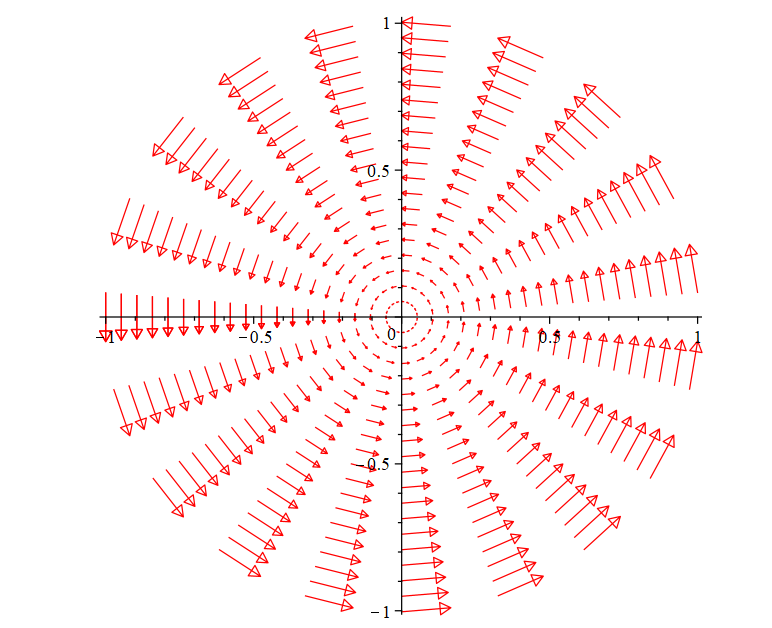
\includegraphics[width=8cm]{exercise13.PNG}
\centering
\caption{Plot representing magnetic field $B_\theta$ of case where where $r < R$}
\end{figure}
 \\
 Here in figure 2 we see that the magnetic field vectors increases with the radius. This is because the magnetic field $B_\theta$ is directly proportional to $r$, as shown in the equation for $B_{i}\left(r\right)$.
\newpage
\\
Then, plotting for $B_{\theta}=\frac{\mu_{0}I}{2\pi \mathrm{r}}$:
\begin{figure}[h!]
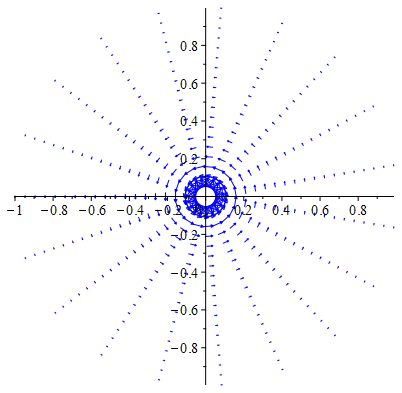
\includegraphics[width=8cm]{halbach_magfield2.png}
\centering
\caption{Plot representing magnetic field of case where $B_\theta$ where $r > R$}
\end{figure}
\\
In figure 3 we see that the magnetic field vectors decrease with the radius, the opposite of the previous vector field. This is because the magnetic field $B_\theta$ is inversely proportional to $r$ (or directly proportional to $\frac{1}{r}$), as shown in the equation for $B_{o}\left(r\right)$

\section{A Halbach Magnet}
In the following exercises we will use our understanding of the behaviour of magnetic fields to study the Halbach magnet more specifically. Essentially, this magnet is a ring composed of magnetic material with a hole in the middle and air surrounding it. 

\subsection{Exercise 14}
To visualize equation 26 from the given exercises,
\begin{equation}
    B_{\mathit{rem}}=\left[\begin{array}{c}
B_{\mathit{rem},r} 
\\
 B_{\mathit{rem},\theta} 
\end{array}\right]=B_{\mathit{rem}}\left[\begin{array}{c}
\cos\left(p\mathit{\theta}\right) 
\\
 \sin\left(p\mathit{\theta}\right) 
\end{array}\right]
\end{equation}
First plotting where $p > 0$,
\begin{figure}[h]
\subfig{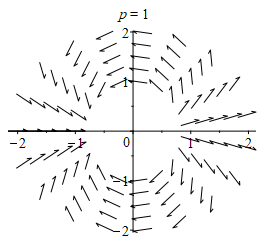
\includegraphics[width=5cm]{halbach_fieldplot_p1.png}}
\subfig{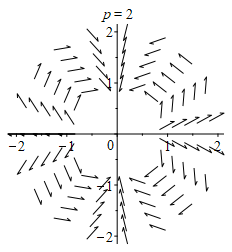
\includegraphics[width=5cm]{halbach_fieldplot_p2.png}}
\subfig{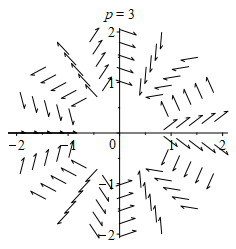
\includegraphics[width=5cm]{halbach_fieldplot_p3.png}}
\centering
\caption{Plots where $B_{rem}$ when $p$ is a positive integer.}
\end{figure}
\newpage
\\
Then plotting where $p < 0$,
\begin{figure}[h]
\subfig{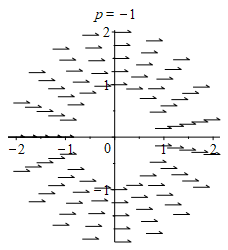
\includegraphics[width=5cm]{halbach_fieldplot_p-1.png}}
\subfig{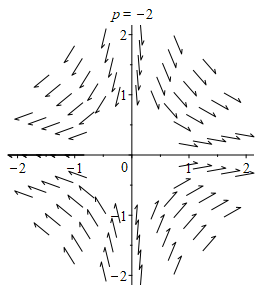
\includegraphics[width=5cm]{halbach_fieldplot_p-2.png}}
\subfig{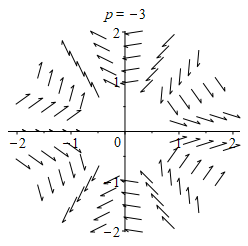
\includegraphics[width=5cm]{halbach_fieldplot_p-3.png}}
\centering
\caption{Plots where $B_{rem}$ when $p$ is a negative integer.}
\end{figure}
\\
All of the above magnetic field plots correspond to the magnetic field of a Halbach magnet. These fields consist of a bore represented by the empty space in the middle, that is surrounded by magnetic field arrows that together are shaped like a circle around the bore (For plots, see appendix 5). 
\\
\\
The first three plots (displayed in figure 4) are with positive values for $p$. These plots are all internal fields, as that the magnetic field lines are directed towards the bore. This is a characteristic of remanence (defined in the text as the magnetic induction remaining in a magnetized substance that is no longer under external magnetic influence) when $p$ is a positive integer.
\\
\\
In contrast, the last three plots (displayed in figure 5) are with negative values for $p$. These plots are all external fields, as that the magnetic field lines are directed away from the bore. This is a characteristic of remanence when $p$ is a negative integer.
\\
\\
Furthermore, $p$ represents $\frac{\mathrm{poles}}{2}$, the number of times that the magnetic field enters or exits the bore. This shows that these graphs are of dipole magnets.



\subsection{Exercise 15}
To show that $\mathbf{Rot}(\nabla f) = 0$ with $f \in  \mathbb{R}$, we can use the definition of a gradient, as mention before, as well as our answer from exercise 2 to know that:
\begin{equation}
    \nabla f\left(x,y,z\right) = (\frac{\partial f}{\partial x},\frac{\partial f}{\partial y},\frac{\partial f}{\partial z})
\end{equation}
Now following 26.25 from the eNotes, it is known that $\mathbf{Rot}(\nabla f) = \nabla \times \nabla f$.
\\
This is then evaluated out to be:
\begin{equation}
    \mathbf{Rot}(\nabla f) = 
\left[\begin{array}{c}
\frac{\partial}{\partial x} 
\\
 \frac{\partial}{\partial y} 
\\
 \frac{\partial}{\partial z} 
\end{array}\right]
\times 
\left[\begin{array}{c}
\frac{\partial f}{\partial x} 
\\
 \frac{\partial f}{\partial y} 
\\
 \frac{\partial f}{\partial z} 
\end{array}\right]
=
\left[\begin{array}{c}
\frac{\partial}{\partial y}\frac{\partial f}{\partial z}-\frac{\partial}{\partial z}\frac{\partial f}{\partial y} 
\\
 \frac{\partial}{\partial z}\frac{\partial f}{\partial x}-\frac{\partial}{\partial x}\frac{\partial f}{\partial z} 
\\
 \frac{\partial}{\partial x}\frac{\partial f}{\partial y}-\frac{\partial}{\partial y}\frac{\partial f}{\partial x} 
\end{array}\right]
=
\left[\begin{array}{c}
0 
\\
 0 
\\
 0 
\end{array}\right]
\end{equation}
This thus proves that $\mathbf{Rot}(\nabla f) =  0$.
\subsection{Exercise 16}
It is given that $A=A_{0}+\nabla f$
\\
If we then find the divergence of each component in the above equation, the equation becomes:
\begin{equation}
    \mathbf{Div(A)}=\mathbf{Div}(A_0)+\mathbf{Div}(\nabla f)
\end{equation}
If any function $f$ is chosen for which $\mathbf{Div(A) = 0}$, we see that $0=\mathbf{Div(A_0)}+\mathbf{Div}(\nabla f)$ which can be rewritten as $\mathbf{-Div(A_0)}=\mathbf{Div}(\nabla f)$.
\\
If the curl of each component in the above equation is found, the equation becomes:
\begin{equation}
    \mathbf{Rot(A)} = \mathbf{Rot(A_0)}+ \mathbf{Rot}(\nabla f)
\end{equation}
Since it was demonstrated in exercise 15 that $\mathbf{Rot}(\nabla f) = 0$, this equation can be rewritten as:
\begin{equation}
    \mathbf{Rot(A)} = \mathbf{Rot(A_0)}
\end{equation}
This equation subsequently defines the curl of $\mathbf{A}$:
\begin{equation}
    \mathbf{Curl(A)} = \mathbf{Curl(A_0)}
\end{equation}
\subsection{Exercise 17}
In this exercise, it is asked that the curl of $B$ from equations 29-30 given in the exercises is found. 
\\
As given by line 29 in exercise 14, one can observe the relationship between the magnetic field $B$ and magnetic potential $A$ as $\mathbf{B}=\mathbf{Rot(A)}$. From this, the curl of both sides can be taken to find $\mathbf{Rot(B)} = \mathbf{Rot(Rot(A))}$. 
Then, using the definition of a curl from eNote 26, definition 26.25, this can be rewritten as:
\begin{equation}
    \mathbf{Rot(Rot(A))} = \nabla \times \left(\nabla \times A\right)
\end{equation}
This equation subsequently can be equated to a vector identity such that:
\begin{equation}
    \nabla \times \left(\nabla \times A\right) = \left\nabla(\nabla A\right)-\nabla ^{2}A
\end{equation}
From exercise 16 it is understood that $\nabla A$ is 0, meaning that this equation becomes:
\begin{equation}
    \nabla \times \left(\nabla \times A\right) = -\nabla ^{2}A
\end{equation}                        
Thus, the curl of $\mathbf{B}$ can be defined as:
\begin{equation}
    \mathbf{Rot(B)} = -\nabla ^{2}A
\end{equation} 
\subsection{Exercise 18}
To again visualize equation 26 from the given exercises, it can be written as:
\begin{equation}
    B_{\mathit{rem}}=\left[\begin{array}{c}
B_{\mathit{rem},r} 
\\
 B_{\mathit{rem},\theta} 
\end{array}\right]=B_{\mathit{rem}}\left[\begin{array}{c}
\cos\left(p\mathit{\theta}\right) 
\\
 \sin\left(p\mathit{\theta}\right) 
\end{array}\right]
\end{equation}
Modelling after the equation in line 21 in the given exercises, $\mathbf{Rot(B)}$ can be found to be: 
\begin{equation}
    \mathbf{Rot(B)}=\left(\frac{1}{r}\frac{\partial B_{z}}{\partial \theta}-\frac{\partial B_{\theta}}{\partial z}\right)\mathbf{e}_{r}+\left(\frac{\partial B_{r}}{\partial z}-\frac{\partial B_{z}}{\partial r}\right)\mathbf{e}_{\theta}+\left(\frac{\partial B_{\theta}}{\partial r}+\frac{B_{\theta}}{r}-\frac{1}{r}\frac{\partial B_{r}}{\partial \theta}\right)\mathbf{e}_{z}
\end{equation}
In addition, it is known from line 23 in the given exercises that:
\begin{equation}
   \frac{\partial B_{r}}{\partial z}=0,\frac{\partial B_{\theta}}{\partial z}=0,\frac{\partial B_{z}}{\partial z}=0 
\end{equation}
And from equations \ref{eq:70} and \ref{eq:71} exercise 10 we know that:
\begin{equation}
    \frac{\partial B_{z}}{\partial r}=0,\frac{\partial B_{z}}{\partial \theta}=0
\end{equation}
Thus we can further simplify the equation for $\mathbf{Rot(B)}$,
\begin{equation}
   \mathbf{Rot(B)}= \left(\frac{1}{r}\cdot 0-0\right)\mathbf{e}_{r}+\left(0-0\right)\mathbf{e}_{\theta}+\left(\frac{\partial B_{\theta}}{\partial r}+\frac{B_{\theta}}{r}-\frac{1}{r}\frac{\partial B_{r}}{\partial \theta}\right)\mathbf{e}_{z}=\left(\frac{\partial B_{\theta}}{\partial r}+\frac{B_{\theta}}{r}-\frac{1}{r}\frac{\partial B_{r}}{\partial \theta}\right)\mathbf{e}_{z}
\end{equation}
Then using the definition of $\mathbf{B}_{rem}$ from line 26 in the given exercises,
\begin{equation}
    \mathbf{Rot(B_{rem})}=\left(\frac{\partial B_{\mathit{rem}}\sin\left(p\mathit{\theta}\right)}{\partial r}+\frac{B_{\mathit{rem}}\sin\left(p\mathit{\theta}\right)}{r}-\frac{1}{r}\frac{\partial B_{\mathit{rem}}\cos\left(p\mathit{\theta}\right)}{\partial \theta}\right)\mathbf{e}_{z}
\end{equation}
Executing the operations of the equation, it is found that $\frac{\partial \cos\left(p\mathit{\theta}\right)}{\partial \theta}=-\sin\left(p\mathit{\theta}\right)$ and thus 
\begin{equation}
    \mathbf{Rot(B_{rem})}=\left(\frac{\partial B_{\mathit{rem}}\sin\left(p\mathit{\theta}\right)}{\partial r}+\frac{B_{\mathit{rem}}\sin\left(p\mathit{\theta}\right)}{r}-\frac{1}{r}\frac{\partial B_{\mathit{rem}}\cos\left(p\mathit{\theta}\right)}{\partial \theta}\right)\mathbf{e}_{z} = \frac{2B_{\mathit{rem}}\sin\left(p\mathit{\theta}\right)}{r}
\end{equation}
So, it can then be understood that the only non-zero component of $\mathbf{Rot(B_{rem})}$ is $\mathbf{Rot(B_{rem})} \cdot \mathbf{e}_z$ as:
\begin{equation}
    \mathbf{Rot(B_{rem})} \cdot \mathbf{e}_z = \frac{2B_{\mathit{rem}}\sin\left(p\mathit{\theta}\right)}{r}
\end{equation}
\subsection{Exercise 19}
The differential equation 33 from the text is given as:
\begin{equation}
    -\nabla ^{2} A_{z}\left(r,\theta\right)= \mathbf{Rot}\mathbf{\left(B_{\mathit{rem}} \right)\cdot}\mathbf{e}_z
\end{equation}
And from exercise 18 we know that:
\begin{equation}
    \mathbf{Rot(B_{rem})} \cdot \mathbf{e_z} = \frac{2B_{\mathit{rem}}\sin\left(p\mathit{\theta}\right)}{r}
\end{equation}
Therefore the equation line 33 from the given exercises can be rewritten as:
\begin{equation}
    -\nabla ^{2} A_{z}\left(r,\theta\right) = \frac{2B_{\mathit{rem}}\sin\left(p\mathit{\theta}\right)}{r}
\end{equation}
Then, the left hand side of the equation can subsequently be simplified. Following the definition 26.23 from eNote 26, $\nabla ^2$ is defined to take the divergence of the gradient of a function. It is otherwise known as the laplacian operator.
\\
\\
From exercise 8 we know that the divergence equation is:
\begin{equation}
    \mathbf{Div(V)} = \frac{\partial V_{r}}{\partial r}+\frac{V_{r}}{r}+\frac{1}{r}\frac{\partial V_{\theta}}{\partial \theta}+\frac{\partial V_{z}}{\partial z}
\end{equation}
 In addition, it is known from exercise 5 that the gradient is:
 \begin{equation}
     \mathbf{\nabla} f\left(r,\theta,z\right) = \frac{\partial f}{\partial r}\mathbf{e_{r}} + \frac{1}{r}\frac{\partial f}{\partial \theta} \mathbf{e_{\theta}}+\frac{\partial f}{\partial z} \mathbf{e_{z}}
 \end{equation}
Now, the laplacian operator can be applied in terms of cylindrical coordinates.
\begin{equation}
    \nabla ^{2} A_{z}\left(r,\theta\right)=\nabla \cdot \nabla A_{z}\left(r,\theta\right)= \mathbf{Div}\left(\nabla A_{z}\left(r,\theta\right)\right) = 
    \mathbf{Div}\left(\frac{\partial}{\partial r} A_{z}\left(r,\theta\right),\frac{1}{r}\frac{\partial}{\partial \theta} A_{z}\left(r,\theta\right),\frac{\partial}{\partial z}A_{z}\left(r,\theta\right)\right)
\end{equation}
\begin{equation}
=
    \frac{\partial ^{2}}{\partial r\partial r}A_{z}\left(r,\theta\right)+\frac{1}{r}\frac{\partial}{\partial r}A_{z}\left(r,\theta\right)+\frac{1}{r^{2}}\frac{\partial ^{2}}{\partial\theta\partial \theta}A_{z}\left(r,\theta\right)+\frac{\partial ^{2}}{\partial z\partial z}A_{z}\left(r,\theta\right)
\end{equation}
Then, as that $A_z (r, \theta)$ has no $z$-component and is thus therefore independent of $z$, $\frac{\partial^{2}}{\partial z\partial z}A_{z}\left(r,\theta\right)=0$.
Then, applying the negative:
\begin{equation}
    -\nabla ^{2} A_{z}\left(r,\theta\right) = - \frac{\partial ^{2}}{\partial r\partial r}A_{z}\left(r,\theta\right) - \frac{1}{r}\frac{\partial}{\partial r}A_{z}\left(r,\theta\right)-\frac{1}{r^{2}}\frac{\partial ^{2}}{\partial\theta\partial \theta}A_{z}\left(r,\theta\right)-\frac{\partial ^{2}}{\partial z\partial z}A_{z}\left(r,\theta\right)
\end{equation}
Now, substituting in the equation for $A_{z}(r ,\theta)$ from line 34 in the given text (see calculations in appendix 6) we get:
\begin{equation}
    \frac{2B_{\mathit{rem}}\sin\left(p\mathit{\theta}\right)}{r}=\frac{2B_{\mathit{rem}}\sin\left(p\mathit{\theta}\right)}{r}
\end{equation}
This thus verifies the equation and that $A_{z}\left(r,\theta\right)$ is a solution to the differential equation in line 33 of the given exercises. 


\subsection{Exercise 20}
Before getting into this exercise, we would like to present the following drawing of the relevant domains, given in the paper:
\begin{figure}[h!]
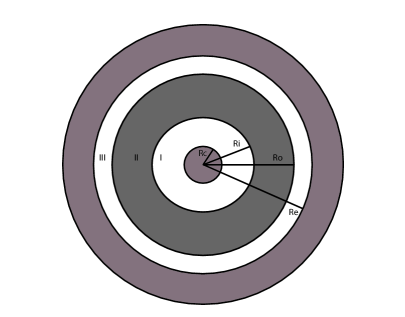
\includegraphics[width=8cm]{zones.PNG}
\centering
\caption{Drawing of the relevant domain for the solution.}
\end{figure}
\\
This figure is what we are going to be using for throughout the next few exercises. In this picture, the Halbach magnet is placed in the grey area, between $r=R_{i}$ and $r=R_{o}$.
\\
\\
For exercise 20, we are asked to find the components of the vector field for $B$ and $H$. 
\\
It is known that $\mathbf{B} = \mathbf{Rot(A)}$ and from equation 21 we know that:
\begin{equation}
    \mathbf{Rot(A)} = \left(\frac{1}{r}\frac{\partial A_{z}}{\partial \theta}-\frac{\partial A_{\theta}}{\partial z}\right)\mathbf{e}_{r}+\left(\frac{\partial A_{r}}{\partial z}-\frac{\partial A_{z}}{\partial r}\right)\mathbf{e}_{\theta}+\left(\frac{\partial A_{\theta}}{\partial r}+\frac{A_{\theta}}{r}-\frac{1}{r}\frac{\partial A_{r}}{\partial \theta}\right)\mathbf{e}_{z}
\end{equation}
But because it is known that $A_r$ only has components in the $z$-direction, we can further simplify this equation to be:
\begin{equation}
\mathbf{Rot(A)} = \frac{1}{r}\cdot \frac{\partial}{\partial \theta}\left(A_{z}\right)\cdot \mathbf{e}_{r}-\frac{\partial}{\partial r}\left(A_{z}\right)\cdot \mathbf{e}_{\theta}=\left[\begin{array}{c}
\frac{1}{r}\cdot \frac{\partial}{\partial \theta}\left(A_{z}\right) 
\\
 -\frac{\partial}{\partial r}\left(A_{z}\right) 
\\
 0 
\end{array}\right]
\end{equation}
Which can thus be rewritten as:
\begin{equation}
   \mathbf{Rot(A)} =  \mathbf{B}=\left[\begin{array}{c}
B_{r} 
\\
 B_{\theta} 
\\
 B_{z} 
\end{array}\right]=\left[\begin{array}{c}
\frac{1}{r}\cdot \frac{\partial}{\partial \theta}\left(A_{z}\right) 
\\
 -\frac{\partial}{\partial r}\left(A_{z}\right) 
\\
 0 
\end{array}\right]
\end{equation}
Then, the value for $A_z$ given in line 34 of the exercises can be substituted in to get (see appendix 7, subsection 1):
\begin{equation}
    B_{r} = \frac{\cos(\theta) \left(-B_{\mathit{rem}} r^{2} \ln (r)+C \,r^{2}+\mathrm{D}\right)}{r^{2}}
\end{equation}    
\begin{equation}
    B_{\theta} = -\sin \left(\theta\right) \left(-B_{\mathit{rem}} \ln\! \left(r\right)+C-B_{\mathit{rem}}\right)+\frac{\sin\! \left(\theta\right) \mathrm{D}}{r^{2}}
\end{equation}
Now, we can insert the value for B given in line 35 of the exercise text to find the components of H (see appendix 7, subsection 2):
\begin{equation}
    H_r= \frac{-B_{\mathit{rem}} \cos \left(p \theta\right) r^{2}+\cos \left(\theta\right) \left(-B_{\mathit{rem}} r^{2} \ln \left(r\right)+C \,r^{2}+\mathrm{D}\right)}{r^{2} \mu_{0} \mu_{r}}
\end{equation}
\begin{equation}
    H_\theta = \frac{-B_{\mathit{rem}} \sin \left(p \theta\right) r^{2}-\sin \left(\theta\right) \left(-B_{\mathit{rem}} r^{2} \ln \left(r\right)+\left(C-B_{\mathit{rem}}\right) r^{2}-\mathrm{D}\right)}{r^{2} \mu_{0} \mu_{r}}
\end{equation}
\begin{equation}
    H_{z}=0
\end{equation}
\subsection{Exercise 21}
Following the example equation at the end of exercise 20 but with consideration of the conditions set in line 37 of the given exercises, it is found that:
\begin{equation}
    \cos\left(\theta\right)\left(C^{\mathit{II}}+\mathrm{D}^{\mathit{II}}R_{o}^{-2}-B_{\mathit{rem}}\ln\left(R_{o}\right)\right)=\cos\left(\theta\right)\left(C^{\mathit{III}}+\mathrm{D}^{\mathit{III}}R_{o}^{-2}\right)
\end{equation}
This equation can only hold true if and only if:
\begin{equation}
    -B_{\mathit{rem}}\ln\left(R_{o}\right)=-C^{\mathit{II}}-\mathrm{D}^{\mathit{II}}R_{o}^{-2}+C^{\mathit{III}}+\mathrm{D}^{\mathit{III}}R_{o}^{-2}
\end{equation}
This can be simplified to the expression:
\begin{equation}
    B_{\mathit{rem}}=\frac{C^{\mathit{II}}R_{o}^{2}+\mathrm{D}^{\mathit{II}}-C^{\mathit{III}}R_{o}^{2}-\mathrm{D}^{\mathit{III}}}{R_{o}^{2}\ln\left(R_{o}\right)}
\end{equation}
\subsection{Exercise 22}
In this exercise, it is asked that we write similar expressions for $C^I$ and $C^{III}$ using components of the vector field from exercise 20 and the boundary conditions for $H_\theta$. It is known from exercise 20 that $B_{rem}$ is a non-zero value only in domain II. 
\\
For domain I:
\\
We firstly follow the equation given in the exercises in line 38:
\begin{equation}
    H_{\theta}^{I}=0|r=R_{c}
\end{equation}
Then applying the condition for $H_\theta$ found for $H_\theta$ in the text for exercise 20,
\begin{equation}
    -\frac{\left(C^{{I}}R_{c}^{2}-\mathrm{D}^{I}\right)\sin\left(\theta\right)}{R_{c}^{2}\cdot \mu_{0}}=0
\end{equation}
Then, after simplifying and rearranging for $C^I$:
\begin{equation}
    C^{I}=\frac{\mathrm{D}^{I}}{R_{c}^{2}}
\end{equation}
\\
For domain I-II:
\\
The third condition (from equation 39 in the given exercises) can subsequently be applied:
\begin{equation}
    H_{\theta}^{I}=H_{\theta}^{\mathit{II}}|r=R_{i}
\end{equation}

Thus,
\begin{equation}
   -\frac{\left(C^{I}R_{i}^{2}-\mathrm{D}^{I}\right)\sin\left(\theta\right)}{R_{i}^{2}\cdot\mu_{0}} = 
\end{equation}
\begin{equation}
    \frac{-B_{\textcolor{DarkOrchid}{\mathit{rem}}}\sin\left(\theta\right)R_{i}^{2}-\sin\left(\theta\right)\left(-B_{\mathit{rem}}\ln\left(R_{i}^{}\right)R_{i}^{2}+R_{i}^{2}\left(C^{\textcolor{DarkOrchid}{\mathit{II}}}-B_{\mathit{rem}}^{}\right)-\mathrm{D}_{}^{\mathit{II}}\right)}{R_{i}^{2}\mu_{\textcolor{DarkOrchid}{0}}\mu_{r}^{\mathit{II}}}
\end{equation}
For domain II-III:
\\
The fourth condition (from equation 40 in the given exercises) can be applied:
\begin{equation}
H_{\theta}^{\mathit{II}}=H_{\theta}^{\mathit{III}}| r =R_{o}
\end{equation}
Thus,
\begin{equation}
    \frac{-B_{\mathit{rem}}\sin\left(\theta\right)R_{o}^{2}-\sin\left(\theta\right)\left(-B_{\mathit{rem}}\ln\left(R_{o}^{}\right)R_{o}^{2}+R_{o}^{2}\left(C^{\mathit{II}}-B_{\mathit{rem}}^{}\right)-\mathrm{D}_{}^{\mathit{II}}\right)}{R_{o}^{2}\mu_{0}\mu_{r}^{\mathit{II}}}
\end{equation}
\begin{equation}
    = \frac{-\left(C^{\mathit{III}}R_{o}^{2}-\mathrm{D}_{}^{\mathit{III}}\right)\sin\left(\theta\right)}{R_{o}^{2}\cdot \mu_{0}}
\end{equation}
Lastly, in regards to domain III:
\\
The fifth and final condition (from equation 41 in the given exercises) can be applied:
\begin{equation}
H_{\theta}^{\mathit{III}}=0| r =R_{e}
\end{equation}
Thus,
\begin{equation}
    \frac{-\left(C^{\mathit{III}}R_{e}^{2}-\mathrm{D}_{}^{\mathit{III}}\right)\sin\left(\theta\right)}{R_{e}^{2}\cdot\mu_{0}}=0
\end{equation}



\subsection{Exercise 23}
To create the matrix asked, we shall use the following six equations, where the first one is given in line 42 of the given exercise text and the others are found and rearranged from our work in exercises 21 and 22:
\\
\\
#1. $C^{\mathrm{I}}+\frac{\mathrm{D}^{\mathrm{I}}}{R_{i}^{2}}-C^{\mathit{II}}-\frac{\mathrm{D}^{\mathit{II}}}{R_{i}^{2}}=-B_{\mathit{rem}} \ln\ \left(R_{i}\right)$
\\
#2. $-C^{\mathit{II}}-\frac{\mathrm{D}^{\mathit{II}}}{R_{o}^{2}}+C^{\mathit{III}}+\frac{\mathrm{D}^{\mathit{III}}}{R_{o}^{2}}=-B_{\mathit{rem}} \ln\ \left(R_{o}\right)$
\\
#3. $-C^{\mathrm{I}}+\frac{\mathrm{D}^{\mathrm{I}}}{R_{c}^{2}}=0$
\\
#4. $-C^{\mathit{III}}+\frac{\mathrm{D}^{\mathit{III}}}{R_{e}^{2}}=0$ 
\\
#5. $-C^{\mathrm{I}} \mu_{r}+\frac{\mathrm{D}^{\mathrm{I}} \mu_{r}}{R_{i}^{2}}+C^{\mathit{II}}-\frac{\mathrm{D}^{\mathit{II}}}{R_{i}^{2}}=B_{\mathit{rem}} \ln\! \left(R_{i}\right)$
\\
#6. $C^{\mathit{II}}-\frac{\mathrm{D}^{\mathit{II}}}{R_{o}^{2}}-C^{\mathit{III}} \mu_{r}+\frac{\mathrm{D}^{\mathit{III}} \mu_{r}}{R_{o}^{2}}=B_{\mathit{rem}} \ln\! \left(R_{o}\right)$
\\
\\
This system of six equations with six unknowns can thus be written into a matrix:
\begin{equation}
\left[\begin{array}{cccccc}
1 & -1 & 0 & \frac{1}{R_{i}^{2}} & -\frac{1}{R_{i}^{2}} & 0 
\\
 0 & -1 & 1 & 0 & -\frac{1}{R_{o}^{2}} & \frac{1}{R_{o}^{2}} 
\\
 -1 & 0 & 0 & \frac{1}{R_{c}^{2}} & 0 & 0 
\\
 0 & 0 & -1 & 0 & 0 & \frac{1}{R_{e}^{2}} 
\\
 -\mu_{r}^{} & 1 & 0 & \frac{\mu_{r}^{}}{R_{i}^{2}} & -\frac{1}{R_{i}^{2}} & 0 
\\
 0 & 1 & -\mu_{r}^{} & 0 & -\frac{1}{R_{o}^{2}} & \frac{\mu_{r}^{}}{R_{o}^{2}} 
\end{array}\right]
\left[\begin{array}{c}
C^{\textcolor{DarkOrchid}{I}} 
\\
 C^{\mathit{II}} 
\\
 C^{\mathit{III}} 
\\
 \mathrm{D}^{I} 
\\
 \mathrm{D}^{\mathit{II}} 
\\
 \mathrm{D}^{\mathit{III}}
\end{array}\right]
= \left[\begin{array}{c}
-B_{\mathit{rem}}\ln\left(R_{i}\right) 
\\
 -B_{\mathit{rem}}\ln\left(R_{o}\right) 
\\
 0 
\\
 0
\\
 B_{\mathit{rem}}\ln\left(R_{i}\right) 
\\
 B_{\mathit{rem}}\ln\left(R_{o}\right) 
\end{array}\right]
\end{equation}

\subsection{Exercise 24}
In this exercise we are asked to find the six constants, $C^I, C^{II}, C^{III}, D^{I}, D^{II}, D^{III}$. In order to find these values, we take the inverse of the matrix we found in exercise 23 and multiplied it by the solution of matrix equation. 
\\
\\
Due to the length of our results, the solution for each constants can be found in the appendix 9, subsection 2 and are separated by commas. The solution is found under the command called "res".

\subsection{Exercise 25}
To show that the equations found in exercise 24 are  equivalent to equations 45-50 given in the text, we can subtract our expression for the 6 constants from our found expressions in our solution (appendix 10). 
\\
As that all of these subtractions equal to 0, it can be deduced that the results obtained through our calculations are identical to those given. 

\subsection{Exercise 26}
Our objective now is to show that a (shown below) is equal to 1 when $R_e$ tends towards infinity and that b (shown below) is equal to -1 when $R_c$ tends towards 0. 
\begin{equation}
    b = \frac{R_{e}^{2}-R_{o}^{2}}{R_{e}^{2}+R_{o}^{2}}
\end{equation}
\begin{equation}
   a = -\frac{-R_{c}^{2}+R_{i}^{2}}{R_{c}^{2}+R_{i}^{2}}
\end{equation}
For a, when $R_e$ tends towards infinity, the difference between $R_e$ and $R_o$ becomes infinitely larger, thus rendering $R_o$ negligible in comparison to $R_e$, thus: 
\begin{equation}
    \underset{R_{e}\rightarrow\infty}{\mathrm{lim}}\left(\frac{R_{e}^{2}-R_{o}^{2}}{R_{e}^{2}+R_{o}^{2}}\right)=\underset{R_{e}\rightarrow\infty}{\mathrm{lim}}\left(\frac{\infty^{2}-R_{o}^{2}}{\infty^{2}+R_{o}^{2}}\right)=1
\end{equation}
In regards to b, when $R_o$ tends towards 0, it becomes negligible, thus:
\begin{equation}
    \underset{R_{c}\rightarrow0}{\mathrm{lim}}\left(-\frac{R_{i}^{2}-R_{c}^{2}}{R_{i}^{2}+R_{c}^{2}}\right)=\underset{R_{c}\rightarrow0}{\mathrm{lim}}\left(-\frac{R_{i}^{2}-0}{R_{i}^{2}+0}\right)=\underset{R_{c}\rightarrow0}{\mathrm{lim}}\left(-\frac{R_{i}^{2}}{R_{i}^{2}}\right)=-1
\end{equation}
\subsection{Exercise 27}
To find the limit of of the constant $D^{II}$ when $\mu_r$ approaches 1 for a single Halbach Magnet in air where $D^{II}$ is defined in equation 45 of the given text,
\begin{equation}
    \underset{{R_{e}\rightarrow\infty}}{\mathrm{lim}}\left(\underset{R_{c}\rightarrow0}{\mathrm{lim}}\left(\underset{\mu_{r}\rightarrow1}{\mathrm{lim}}\mathrm{D}^{\mathit{II}}\right)\right)
\end{equation}
When solved (see appendix 12), this is found to be:
\begin{equation}
    0
\end{equation}
\subsection{Exercise 28}
Now finding the limits of the constants $C^{II}, D^{III},$ and $C^{III}$ using the same limits in exercise 27:
\\
For $C^{II}$ defined in equation 48:
\begin{equation}
  \underset{{R_{e}\rightarrow\infty}}{\mathrm{lim}}\left(\underset{R_{c}\rightarrow0}{\mathrm{lim}}\left(\underset{\mu_{r}\rightarrow1}{\mathrm{lim}}C^{\mathit{II}}\right)\right)
\end{equation}
When solved, (see appendix 13, subsection 1) this is found to be:
\begin{equation}
    B_{rem}\ln{(R_{0})}
\end{equation}
For $C^{III}$:
\begin{equation}
  \underset{{R_{e}\rightarrow\infty}}{\mathrm{lim}}\left(\underset{R_{c}\rightarrow0}{\mathrm{lim}}\left(\underset{\mu_{r}\rightarrow1}{\mathrm{lim}}C^{\mathit{III}}\right)\right)
\end{equation}
When solved, (see appendix 13, subsection 2) this is found to be:
\begin{equation}
    0
\end{equation}
For $D^{III}$:
\begin{equation}
  \underset{{R_{e}\rightarrow\infty}}{\mathrm{lim}}\left(\underset{R_{c}\rightarrow0}{\mathrm{lim}}\left(\underset{\mu_{r}\rightarrow1}{\mathrm{lim}}D^{\mathit{III}}\right)\right)
\end{equation}
When solved, (see appendix 13, subsection 3) this is found to be:
\begin{equation}
    0
\end{equation}
\subsection{Exercise 29}
Now lastly finding the limits of $C^I$ and $D^I$ (as defined in equations 46 and 47 in the text) when $\mu_r$ approaches 1,
\\
\\
For $C^I$,
\begin{equation}
  \underset{{R_{e}\rightarrow\infty}}{\mathrm{lim}}\left(\underset{R_{c}\rightarrow0}{\mathrm{lim}}\left(\underset{\mu_{r}\rightarrow1}{\mathrm{lim}}C^{\mathit{I}}\right)\right)
\end{equation}
When solved, (see appendix 14) this is found to be:
\begin{equation}
    -B_{rem}\ln{(\frac{R_i}{R_\theta})}
\end{equation}
For $D^I$,
\begin{equation}
  \underset{{R_{e}\rightarrow\infty}}{\mathrm{lim}}\left(\underset{R_{c}\rightarrow0}{\mathrm{lim}}\left(\underset{\mu_{r}\rightarrow1}{\mathrm{lim}}D^{\mathit{I}}\right)\right)
\end{equation}
When solved, (see appendix 14) this is thus found to be:
\begin{equation}
    0
\end{equation}
\subsection{Exercise 30}
In this exercise we are asked to show graphically how the norm $B = 
\sqrt{B_{r}^{2}+B_{\theta}^{2}}$ behaves. Knowing that $B_{rem}$ (remanence) can only be found where the permanent magnet is situated and $R_{i}$ and $R_{o}$ is the interval that defines the region where the magnet can be found, we have to analyse domain II. With the given value for $B_{rem}=1.4$T and assuming that our $R_{o}=5$, we have the following equation for the area of the magnet (see appendix 15):
\begin{equation}
    A = 
\sqrt{ 1.96 \ln \! \left(\frac{5}{r}\right)^{2} \left(\cos^{2}\left(\theta \right)\right)+ 1.96 \left(\sin^{2}\left(\theta \right)\right) \left(\ln \! \left(\frac{5}{r}\right)-1\right)^{2}}
\end{equation}
Using this equation, it can be displayed visually as the following contour plot: 
\begin{figure}[h!]
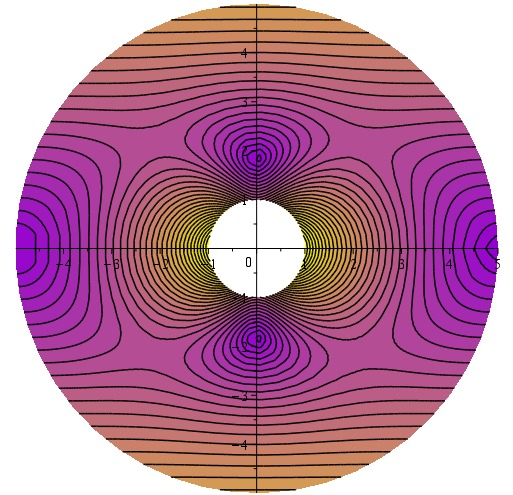
\includegraphics[width=8cm]{imagem_ex_30.jpeg}
\centering
\caption{Magnetic field inside of the magnet}
\end{figure}
\\
The above magnetic field represented in the graph displays the varying strength of the magnetic field inside of the Halbach magnet. The colors range from from violet to yellow where the violet represents the strongest parts of the magnetic field and the yellow represents the weakest parts of the magnetic field. 
\subsection{Exercise 31}
Using the equations given in lines 53 and 54, we can formulate the equation for B in the first domain following the structure of $B = \sqrt{B^2_r + B^2_\theta}$
\\
\begin{equation}
    B=\sqrt{\left(B_{\mathit{rem}}\ln\left(\frac{R_{o}}{R_{i}}\right)\cos\left(\theta\right)\right)^{2}+\left(-B_{\mathit{rem}}\ln\left(\frac{R_{o}}{R_{i}}\right)\sin\left(\theta\right)\right)^{2}}
\end{equation}
This can subsequently be simplified using the Pythagorean trigonometric identity:
\begin{equation}
    B=\sqrt{B_{\mathit{rem}}^{2}\ln\left(\frac{R_{o}}{R_{i}}\right)^{2}}   
\end{equation}
Simplifying further,
\begin{equation}
   B=B_{\mathit{rem}}^{}\ln\left(\frac{R_{o}}{R_{i}}\right)
\end{equation}
This equation will always hold true if being equal to a value greater than 0. For this to be true, the following conditions must be met:
\begin{equation}
    R_{o}\neq 0
\end{equation}
\begin{equation}
    R_{i}\neq0
\end{equation}
\\
The expression for the magnitude of the magnetic field outside of the conductor with our values for $B_{rem}$ and $B_i$ inserted, thus $B$ is defined as $B = \sqrt{ 1.96 \cos \left(A\theta\right)^{2} \ln \left(\frac{R_{o}}{5}\right)^{2}+ 1.96 \sin \left(\theta\right)^{2} \ln \left(\frac{R_{o}}{5}\right)^{2}}\colon$
\\
\\
\begin{figure}[h!]
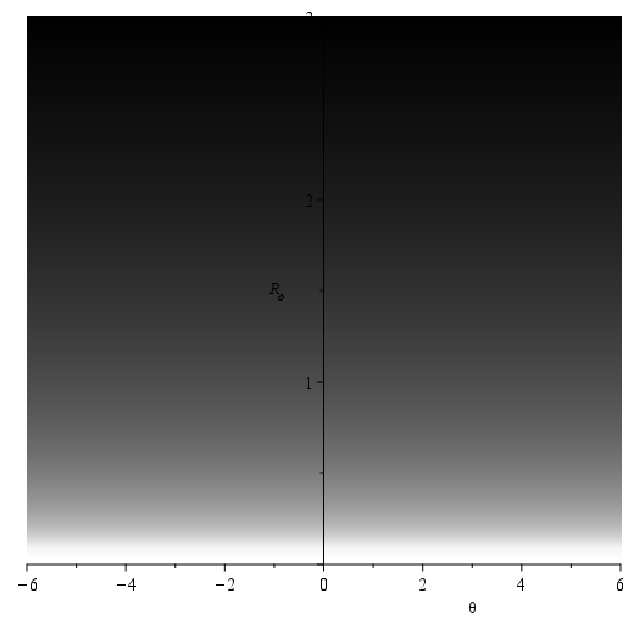
\includegraphics[width=8cm]{exercise31__1.PNG}
\centering
\caption{Representation of the strength of the magnetic field outside of the magnet}
\end{figure}
\\
This graph (see appendix 16, subsection 1) represents a magnetic field  outside of the conductor (in domain I) where the white part (located in the center of domain I) represents a low magnetic field and the darker it gets, the higher the magnetic field gets since it gets closer to the inner part of the magnet.
\\
\\
In addition, we can display the behaviour of B in domain I in the form of a contour plot (see appendix 16, subsection 2), where the white part is the middle and the black is the closest region to the magnet:
\begin{figure}[h!]
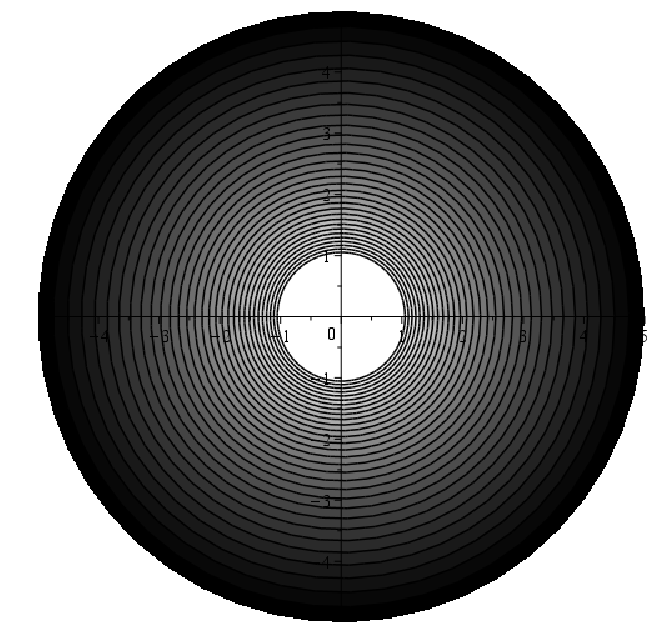
\includegraphics[width=8cm]{exercise31__2.PNG}
\centering
\caption{Contour plot that shows the magnetic field outside of the magnet}
\end{figure}
\section{Halbach magnets and their applications}
Finally, we shall consider applications of Halbach cylinders and how they are utilized in real world situations. One real life example is the MRI machine which requires a large magnetic field. This magnetic field can be induced by a Halbach magnet. Here we compare the efficiency of utilizing a Halbach magnet versus a solenoid coil to create an MRI magnet.  
\subsection{Exercise 32}
From observing the images (a) and (b) we can understand that the current flows inwards. And with utilizing the right hand rule - where one can wrap a hand in the direction of the current and their thumb will point in the direction of the magnetic field- it can be said that the magnetic field points from the right to the left. 
\begin{figure}[h!]
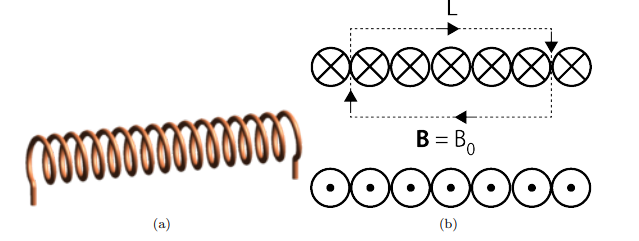
\includegraphics[width=10cm]{exercise32.PNG}
\centering
\caption{Contour plot that shows the magnetic field outside of the conductor }
\end{figure}

\subsection{Exercise 33}
Ampere's law is given in the equation in line 57 from the given text as:
\begin{equation}
    \int_{\textcolor{DarkOrchid}{\mathit{circ}}}^{}\mathbf{B}dl=\mu_{0}I_{\mathit{enclosed}}
\end{equation}
When simplified,
\begin{equation}
    \mathbf{B}=\mu_{0}I_{\mathit{enclosed}}
\end{equation}
With the knowledge that the number of turns in one segment of the coil is defined as $l (\frac{N}{L})$, the current enclosed by the coil as:
\begin{equation} 
    I_{\mathit{enclosed}}=l\left(\frac{N}{L}\cdotI\right)
\end{equation}
The variables in this equation are defined as the following:
\\
\\
$l$ = length of the wire
\\
$N$ = number of windings
\\
$L$ = length of solenoid
\\
\\
Using this information, Ampere's Law can thus be rewritten as:
\begin{equation}
    \mathit{Bl}=\mu_{0}l\left(\frac{N}{L}\cdotI\right)
\end{equation}
This can be furthered simplified by cancelling out the variable $L$ found on both the right and left hand side of the equation. Thus the magnetic field produced by the coil can be written as the function:
\begin{equation}
    B=\frac{\mu_{0}\mathit{NI}}{L}
\end{equation}

\subsection{Exercise 34}
From the problem itself, we are given the following values:
\\
\\
$R_{i} =  0.6 m$
\\
$B =  1.5 T$
\\
$B_{\mathit{rem}} =  1.4 T$
\\
\\
We can plug these values into the equation  calculated in exercise 31:
\begin{equation}
    B = B_{\mathit{rem}} \ln \! \left(\frac{R_{o}}{R_{i}}\right)
\end{equation}
\begin{equation}
    1.5 T =  1.4 T \ln \! \left(\frac{R_{o}}{0.6m}\right)
\end{equation}
Then rearranging this equation to solve for $R_{o}$:
\begin{equation}
    R_{o} = 0.6 m \cdot e^{\frac{1.5T}{1.4T}}
\end{equation}
Finally, this can be simplified to:
\begin{equation}
    R_{o} =  1.751728382 m
\end{equation}

\subsection{Exercise 35}
From the equation solved in exercise 33, it is know that:
\begin{equation}
    B=\frac{\mu_{0} \mathit{NI}}{L}
\end{equation}
\\
The following values are given:
\\
\\
$N=5000$
\\
\\
It is also known that:
\\
\\
$L=0.5m$
\\
$B=1.5T$
\\
\\
Then, we randomly assign a value for $\mu_{0}$:
\begin{equation}
   \mu_{0}=4\pi\cdot \mathit{10}^{-7}\frac{N}{A^{2}}
\end{equation}
Plugging these values into the above equation from exercise 33 and solve for I:
\begin{equation}
    1.5T=\frac{\left(4\pi \cdot \mathit{10}^{-7}\frac{N}{A^{2}}\right)\left(5000\right)I}{ 0.50m}
\end{equation}
From this, the value of the current is found to be:
\begin{equation}
    \mathrm{I}  =  119.366 A
\end{equation}
This result is unrealistic because this value exceeds the realistic maximum amount of current that a 1 mm wire can carry. 

\subsection{Exercise 36}
Because the solenoid will have a 1 mm diameter and a length of 50 cm, we can account for both of these values by putting 10 layers of copper wire with 500 windings for each layer. Every layer would be 1mm thick so that the total thickness would be 1cm - which is negligible compared to a 60cm diameter.
We know that the wire moves in a circular motion, of which the circumference of any circle is given by:
\\
\\
$C = 2 \mathit{\pi r}$
\\
\\
And we've decided that the diameter will be:
\\
$\mathit{diameter} =  0.6 m$
\\
Which means:
\\
$\mathit{radius} =  0.3 m$
\\
\\
Ultimately the length of the copper wire can be given by:
\begin{equation}
    \mathit{lenght} \mathit{of} \mathit{copper} \mathit{wire} = 
    \mathit{circumference} \cdot \mathit{windings} \cdot \mathit{layers}
\end{equation}
Plugging in values, this can be rewritten as:
\begin{equation}
    \mathit{length}\mathit{of}\mathit{copper}\mathit{wire}=2\pi\cdot \mathit{\,0.3}\cdot \mathit{500}\cdot \mathit{10}
\end{equation}
Which approximately equals to:
\begin{equation}
    \mathit{length} \mathit{of} \mathit{copper} \mathit{wire} = 
 9424.777962 m
\end{equation}
\subsection{Exercise 37}
It is given in the question that:
\\
\\
$\rho= 1.68\cdot10^{-8}\Omega\mathrm{m}$
\\
$R=\rho\frac{l}{A}$
\\
\\
Where:
\\
$l$ = length of the wire
\\
$A$ = cross sectional area of cable
\\
\\
In addition, it is known from the given Joule-heating effect that:
\\
\\
$P = I^2 \cdot R$
\\
\\
Where when this is combined with the aforementioned equation for $R$ we find:
\\
\\
$\frac{P}{I^{2}}=\rho\frac{l}{A}$
\\
\\
When rewritten:
\\
\\
$P=I^{2}\rho\frac{l}{A}$
\\
\\
$A$ is defined as $\left( 0.0005\right)^{2}\pi= 7.853981635\times10^{-7}$
\\
$l$ is defined from our solution to exercise 36, $l = 9424.777960m$.
And from exercise 35, it is known $I= 119.366A$.
Inserting these values into our above equation to find the expected heating in the copper wire:
\begin{equation}
    P=\left( 119.366\right)^{2}\cdot\left( 1.68\cdot10^{-8}\right)\cdot\frac{\left( 9424.777960\right)}{\left( 7.853981635\times10^{-7}\right)}
\end{equation}
Thus, we find:
\\
\\
$P = 2.872445578 \cdot 10^6 W$
\\
This is not negligible, as that this is too large of a value to be ignored.
\subsection{Exercise 38}
From the question it is given that:
\\
\\
$I_C(B) = \frac{I_0}{(1 + B/B_0)}$
\\
$B_{0}=3T$
\\
$I_0 = 1.8kA$
\\
\\
Where $B$ = the
magnetic flux density in the bore of the solenoid, and $I_C(B) = I_{enclosed}$ (for the superconductor).
\\
\\
From exercise 33 we know that:
\\
\\
$B=\frac{\mu_{0}\mathit{NI}}{L}$
\\
\\
Substituting this value for $B$ from exercise 33 into the given equation for $I_C(B)$:
\begin{equation}
    I_{C}\left(B\right)=\frac{I_{0}}{\left(1+\frac{\left(\frac{\mu_{0}\mathit{NI}}{L}\right)}{B_{0}}\right)}
\end{equation}
Which can be simplified to:
\begin{equation}
    I_{C}\left(B\right)=\frac{I_{0}B_{0}L}{\left(\mathit{LB}_{0}+\mu_{0}\mathit{NI}\right)}
\end{equation}
Calculating with our known values (see appendix 22), we thus find that:
\\
\\
$I_{c}= 1200A$
\\
$N = 497$ Windings
\newpage
\section{Conclusion}

Throughout this project, we have been studying the math behind Halbach magnets. We started with more general problems of working with cylindrical coordinates. By doing so we had a better understanding of how to manage vector fields in space and a deeper understanding of the basic concepts regarding polar coordinates and vectors themselves. We then moved on to analyzing magnetic fields around a conductor which helped gear our previous work with vector fields more towards permanent magnets. Then to get even more specific, we then worked on problems with Halbach magnets exclusively to observe how different regions of the magnet behave in different situations and the properties they have. In doing so, we studied the magnetic field inside the magnet, and also the outer and inner parts of the exterior magnetic field. We concluded with real-life application of Halbach magnets - observing how they work in MRI machines to ultimately prove our understanding of how they work and how useful they are in the real world.

\section{References}
 1. Søren Enemark, Steen Markvorsen, and Karsten Schmidt. Advanced Engineering Mathematics I Part I Linear Algebra and Differential Equations. January 11, 2022 ed., Technical University of Denmark, 2022.
\\
\\
2. Kaspar K. Nielsen &amp; Rasmus Bjørk. “Analytical Modeling of 2D Halbach Permanent Magnets.” Mar. 2022. \\
\\
3. Kraus, John D., and Keith R. Carver. Electromagnetics. Second Edition. McGraw-Hill Book Co., 1973. 
\end{document}